\documentclass{article}
\usepackage{amsmath,amssymb,listings,upquote}
\usepackage[margin=3cm]{geometry}
\usepackage{graphicx,color}
\lstset{language=Python}
\usepackage{enumerate}% http://ctan.org/pkg/enumerate
\usepackage{fancyvrb}


\newcounter{zone}
\setcounter{zone}{0}
\newcommand{\zone}{\clearpage\refstepcounter{zone}\section*{Zone \arabic{zone}}}
\newcounter{question}
\setcounter{question}{0}
\newcounter{variant}
\newcounter{questionpoints}
\newcommand{\question}[1]{\newpage \refstepcounter{question} \setcounter{variant}{0} \setcounter{questionpoints}{#1}}
\newcommand{\variant}{\vspace{4em}\refstepcounter{variant}\noindent \arabic{question}/\arabic{variant}. (\arabic{questionpoints} point\ifnum \thequestionpoints > 1 s\fi) }
\newenvironment{answers}{\begin{enumerate}}{\end{enumerate}}
\newcommand{\answer}{\item }
\newcommand{\correctanswer}{\item $\bigstar$ }
\renewcommand{\theenumi}{\Alph{enumi}}
\newenvironment{solution}{{\bf Solution.} }{\vspace*{.3in}\hrule}

\begin{document}

\begin{center}
\textbf{\Large CS 101 Practice Final Exam}
%
%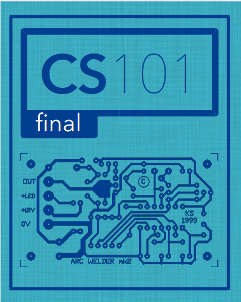
\includegraphics[width=2in]{../img/final-header.png}
\end{center}

\bigskip
\noindent
\begin{itemize}
	\item  \textbf{Be sure to enter your information below, enter your answers for multiple-choice questions on the next page, and your code for the last two coding questions on the last two pages}.  Do not turn this page until instructed to.
	\item  This is a 180-minute exam with 30 questions:
	\begin{itemize}
		\item  12 MATLAB multiple-choice questions worth 5 points each;
		\item  16 Python multiple-choice questions worth 5 points each; and
		\item  2 coding questions worth 30 points each
	\end{itemize}
	for a total of 200 possible points.
	
	\item  \textbf{Your are NOT allowed to take any page of this final exam out of the final exam classroom. In other words, all pages of your final exam must be submitted.}  
	\item  Each multiple choice question has only \emph{one} correct answer.
	\item  You must not communicate with other students during the exam.
	\item No books, notes, or electronic devices are permitted. In other words, you are not allowed to use a dictionary on your mobile phone or other electronic devices. However, if you don't understand the meaning of a particular English word in this exam, please raise your hand and the instructor will explain the meaning of the English word to you. 
\end{itemize}

\bigskip\bigskip
\noindent
\textbf{\Large 1. Fill in your information:}

\bigskip
{\Large\bf
	\begin{tabular}{ll}
		Full Name: & \underbar{\hskip 8cm} \\[0.5em]
		Student ID: & \underbar{\hskip 8cm} \\[0.5em]
		%NetID: & \underbar{\hskip 8cm}
	\end{tabular}
}

%%%%%%%%%%%%%%%%%%%%%%%%%%%%%%%%%%%%%%%%%%%%%%%%%%%%%%%%%%%%%%%%%%%%%%%%%%%%%%%
%%%%%%%%%%%%%%%%%%%%%%%%%%%%%%%%%%%%%%%%%%%%%%%%%%%%%%%%%%%%%%%%%%%%%%%%%%%%%%%
\zone \pagebreak \noindent
\textbf{The following 12 questions involve MATLAB.}
\\\\

%%%%%%%%%%%%%%%%%%%%%%%%%%%%%%%%%%%%%%%%%%%%%%%%%%%%%%%%%%%%%%%%%%%%%%%%%%%%%%%
\question{5}
\variant %---------------------------------------------------------------------
Consider the following MATLAB program:
\begin{Verbatim}
x = [ 1 2 ];
y = [ 3 4 ];
z = [ x' [ y ; y ] ]';
\end{Verbatim}

What is the \textbf{value} of \texttt{z} after this program executes?

\begin{answers}
  \answer $ \left[ \begin{array}{cc} 1 & 2 \\ 3 & 4 \\ 3 & 4 \\ \end{array} \right] $
  \answer $ \left[ \begin{array}{ccc} 1 & 3 & 3 \\ 2 & 4 & 4 \\ \end{array} \right] $
  \answer $ \left[ \begin{array}{ccc} 1 & 3 & 4 \\ 2 & 3 & 4 \\ \end{array} \right] $
  \correctanswer $ \left[ \begin{array}{cc} 1 & 2 \\ 3 & 3 \\ 4 & 4 \\ \end{array} \right] $
  \answer None of the other answers are correct
\end{answers}

\begin{solution}
\end{solution}


%%%%%%%%%%%%%%%%%%%%%%%%%%%%%%%%%%%%%%%%%%%%%%%%%%%%%%%%%%%%%%%%%%%%%%%%%%%%%%%
\question{5}
\variant %---------------------------------------------------------------------
Consider the following MATLAB program:
\begin{Verbatim}
A = ones( 4,4 ) + 2 * eye( 4,4 );
A = A - 2;
A( :,3:4 ) = A( :,3:4 ) + 2;
\end{Verbatim}

What is the \textbf{value} of \texttt{A} after this program executes?

\begin{answers}
  \correctanswer $ \left[ \begin{array}{cccc} 1 & -1 & 1 & 1 \\ -1 & 1 & 1 & 1 \\ -1 & -1 & 3 & 1 \\ -1 & -1 & 1 & 3 \\ \end{array} \right] $
  \answer $ \left[ \begin{array}{cccc} 0 & -2 & 0 & 0 \\ -2 & 0 & 0 & 0 \\ -2 & -2 & 2 & 0 \\ -2 & -2 & 0 & 2 \\ \end{array} \right] $
  \answer $ \left[ \begin{array}{cccc} -1 & -1 & 1 & 1 \\ -1 & -1 & 1 & 1 \\ -1 & -1 & -3 & 1 \\ -1 & -1 & 1 & -3 \\ \end{array} \right] $
  \answer $ \left[ \begin{array}{cccc} 1 & 1 & 3 & 3 \\ 1 & 1 & 3 & 3 \\ 1 & 1 & 3 & 3 \\ 1 & 1 & 3 & 3 \\ \end{array} \right] $
  \answer None of the other answers are correct
\end{answers}

\begin{solution}
\end{solution}


%%%%%%%%%%%%%%%%%%%%%%%%%%%%%%%%%%%%%%%%%%%%%%%%%%%%%%%%%%%%%%%%%%%%%%%%%%%%%%%
\question{5}
\variant %---------------------------------------------------------------------
Consider the following MATLAB function stored in \texttt{prink.m}:
\begin{Verbatim}
function [ f g ] = prink( x,y )
  f = x .^ -0.5;
  g = y + f .* 2;
end
\end{Verbatim}

Which of the following correctly assigns the results of a call to \texttt{prink} \texttt{f} to \texttt{F} and \texttt{g} to \texttt{G}, respectively?

\begin{answers}
  \answer  \texttt{F,G = prink( 2,3 );}
  \answer  \texttt{[ F G ] = prink( [ 2 3 ] );}
  \answer  \texttt{[ F G ] = prink( 2 3 );}
  \answer  \texttt{[ F G ] = prink [ 2 3 ];}
  \correctanswer  \texttt{[ F G ] = prink( 2,3 );}
\end{answers}

\begin{solution}
\end{solution}


%%%%%%%%%%%%%%%%%%%%%%%%%%%%%%%%%%%%%%%%%%%%%%%%%%%%%%%%%%%%%%%%%%%%%%%%%%%%%%%
\question{5}
\variant %---------------------------------------------------------------------
Recollect that MATLAB represents polynomials as an array of coefficients from the highest-order coefficient to the lowest.  For instance,
$$
x^{3} + x + 2
$$
is written as the array \texttt{[ 1 0 1 2 ]}.

How would we represent the summation of the two polynomials
$$
x^{2} + x + 1
$$
and
$$
x^{3} + x^{2} - 1
$$
as a MATLAB polynomial array?

\begin{answers}
  \answer  \texttt{[ 1 1 1 ] + [ 1 1 0 -1 ]}
  \answer  \texttt{[ 1 1 1 ] + [ -1 0 1 1 ]}
  \correctanswer  \texttt{[ 0 1 1 1 ] + [ 1 1 0 -1 ]}
  \answer  \texttt{[ 1 1 1 0 ] + [ 1 1 0 -1 ]}
\end{answers}

\begin{solution}
\end{solution}


%%%%%%%%%%%%%%%%%%%%%%%%%%%%%%%%%%%%%%%%%%%%%%%%%%%%%%%%%%%%%%%%%%%%%%%%%%%%%%%
\question{5}
\variant %---------------------------------------------------------------------
Consider the following two-dimensional MATLAB array, stored in the variable \texttt{A}:
$$
\left[ \begin{array}{ccc}
 1 &   1 \\
 3 &   6 \\
 9 &  36 \\
27 & 216 \\
\end{array} \right]
$$

How can we index and retrieve the value 36 from this array?

\begin{answers}
  \answer  \texttt{A( 2,1 )}
  \correctanswer  \texttt{A( 3,2 )}
  \answer  \texttt{A( 2,3 )}
  \answer  \texttt{A[ 2,1 ]}
  \answer  \texttt{A[ 3,2 ]}
\end{answers}

\begin{solution}
\end{solution}


%%%%%%%%%%%%%%%%%%%%%%%%%%%%%%%%%%%%%%%%%%%%%%%%%%%%%%%%%%%%%%%%%%%%%%%%%%%%%%%
\question{5}
\variant %---------------------------------------------------------------------
\emph{For this problem, you should compose a function which accomplishes a given task using the available code blocks arranged in the correct functional order.}

The Levi-Civita symbol represents a direction of travel through the permutations of the elements of a vector (or higher-order tensor).  For a 3D vector, given numbers $i$, $j$, $k$,
$$
\varepsilon_{ijk} =
\left\{
\begin{bmatrix}
    +1 \hspace{1cm} (1,2,3), (2,3,1), (3,1,2); \\
    -1 \hspace{1cm} (3,2,1), (2,1,3), (1,3,2); \\
    0 \hspace{1cm} \text{if}\, i=j, j=k, \,\text{or}\, k=i.
\end{bmatrix}
\right.
$$

Compose a function \texttt{epsilon} which accepts a vector \texttt{ind} representing the three values $i$, $j$, $k$ in the above definition.  The function should return the value of $\varepsilon_{ijk}$ for those values.

\begin{enumerate}[1]
\item  \texttt{end}  %1
\item  \texttt{s = 0;}  %2
\item  \texttt{s = -1;}  %3
\item  \texttt{s = +1;}  %4
\item  \texttt{if ind(1) == ind(2) | ind(2) == ind(3) | ind(3) == ind(1)}  %5
\item  \texttt{elseif ind(1) == 1 \& ind(2) == 2 \& ind(3) == 3}  %6
\item  \texttt{elseif ind(1) == 2 \& ind(2) == 3 \& ind(3) == 1}  %7
\item  \texttt{elseif ind(1) == 3 \& ind(2) == 1 \& ind(3) == 2}  %8
\item  \texttt{elseif ind(1) < ind(2) \& ind(2) < ind(3) \& ind(3) < ind(1)}  %9
\item  \texttt{function [ s ] = epsilon( ind )}  %10
\item  \texttt{function epsilon( ind )}  %11
\item  \texttt{else}  %12
\item  \texttt{if ind(1) == 1 \& ind(2) == 2 \& ind(3) == 3}  %13
\end{enumerate}

\begin{answers}
  \answer  10, 5, 2, 6, 3, 7, 3, 8, 3, 12, 4, 1
  \correctanswer  10, 5, 2, 6, 4, 7, 4, 8, 4, 12, 3, 1, 1
  \answer  10, 2, 13, 4, 12, 3, 1, 1
  \answer  11, 5, 2, 6, 4, 7, 4, 8, 4, 12, 3, 1
\end{answers}

\begin{solution}
\end{solution}


%%%%%%%%%%%%%%%%%%%%%%%%%%%%%%%%%%%%%%%%%%%%%%%%%%%%%%%%%%%%%%%%%%%%%%%%%%%%%%%
\question{5}
\variant %---------------------------------------------------------------------
Consider the following MATLAB program:

\begin{Verbatim}
s = (2 < 3) & ((2 > 3) | (1 ~= 0))
\end{Verbatim}

What is the final value of \texttt{s}?

\begin{answers}
  \answer  \texttt{True}
  \correctanswer  \texttt{1}
  \answer  \texttt{0}
  \answer  \texttt{false}
\end{answers}

\begin{solution}
\end{solution}


%%%%%%%%%%%%%%%%%%%%%%%%%%%%%%%%%%%%%%%%%%%%%%%%%%%%%%%%%%%%%%%%%%%%%%%%%%%%%%%
\question{5}
\variant %---------------------------------------------------------------------
\begin{Verbatim}
x = eye( 2,2 );
y = [ x(:,1) x(:,2) ];
A = [ x y ; y x ];
\end{Verbatim}

What is the final value of \texttt{A( 1:2,1:2 )}?

\begin{answers}
  \answer  \texttt{[ 0 1 ; 1 0 ]}
  \answer  \texttt{[ 1 1 ; 1 1 ]}
  \answer  \texttt{[ 0 0 ; 0 0 ]}
  \correctanswer  \texttt{[ 1 0 ; 0 1 ]}
\end{answers}

\begin{solution}
\end{solution}


%%%%%%%%%%%%%%%%%%%%%%%%%%%%%%%%%%%%%%%%%%%%%%%%%%%%%%%%%%%%%%%%%%%%%%%%%%%%%%%
\question{5}
\variant %---------------------------------------------------------------------
\begin{Verbatim}
x  = linspace( -1,1,101 );
y1 = exp( x );
y2 = tan( x );
y3 = rand( 1,numel(x) );
\end{Verbatim}

How would you successfully plot all three of these data series as points?  (Assume any given plot format strings are valid.)

\begin{answers}
  \correctanswer
    \begin{Verbatim}
plot( x, y1,'r.', x,y2,'g.', x,y3,'b.' );
    \end{Verbatim}
  \answer
    \begin{Verbatim}
plot( x, y1,'r.', y2,'g.', y3,'b.' );
    \end{Verbatim}
  \answer
    \begin{Verbatim}
hold on;
plot( x, y1 );
plot( x, y2 );
plot( x, y3 );
    \end{Verbatim}
  \answer
    \begin{Verbatim}
plot( x,y1, x,y2, x,y3 );
    \end{Verbatim}
\end{answers}

\begin{solution}
\end{solution}


%%%%%%%%%%%%%%%%%%%%%%%%%%%%%%%%%%%%%%%%%%%%%%%%%%%%%%%%%%%%%%%%%%%%%%%%%%%%%%%
\question{5}
\variant %---------------------------------------------------------------------
Consider the following program, which produces 10,000 random numbers selected from a certain distribution and plots them:
\begin{Verbatim}
x = randn( 10000,1 );
plot( x,'k.' );
\end{Verbatim}

Which of the following plots could result from executing this program?

\begin{answers}
  \answer
    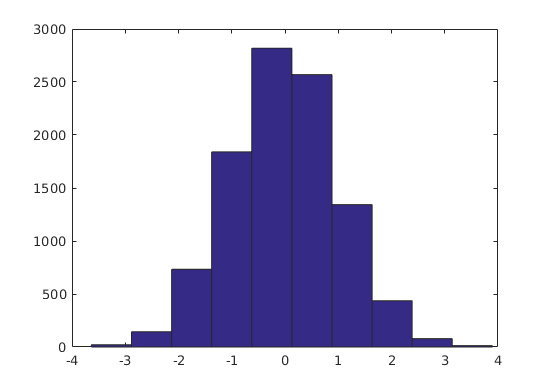
\includegraphics[width=0.4\textwidth]{./hist-normal.png}
  \correctanswer
    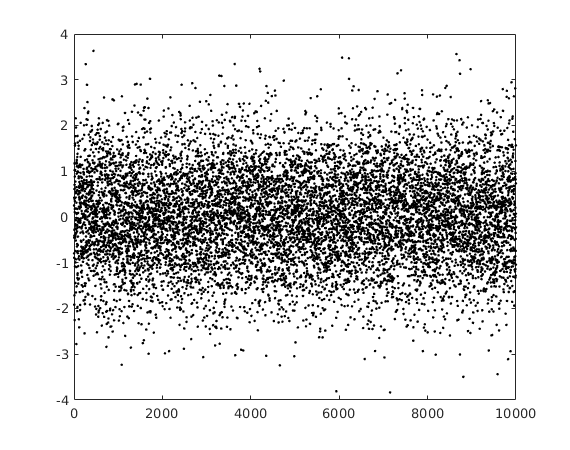
\includegraphics[width=0.4\textwidth]{./plot-normal.png}
  \answer
    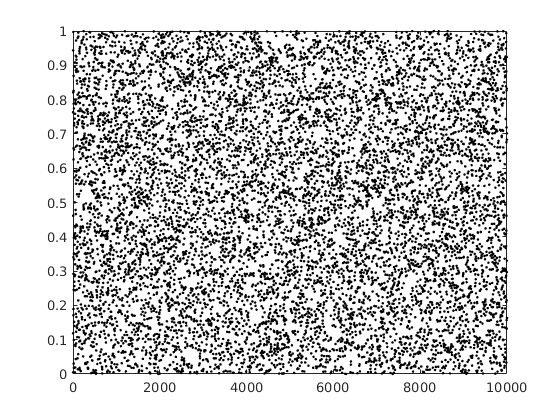
\includegraphics[width=0.4\textwidth]{./plot-uniform.png}
  \answer
    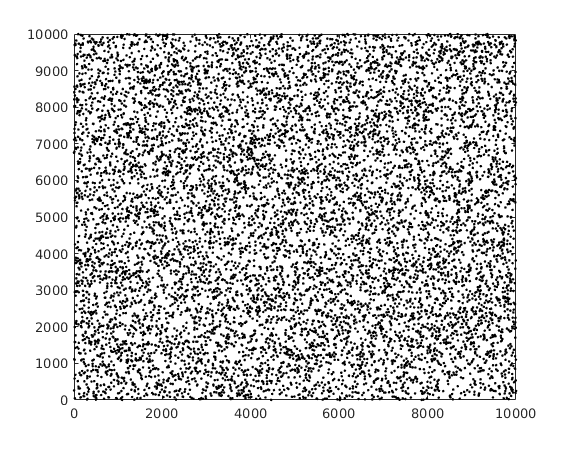
\includegraphics[width=0.4\textwidth]{./plot-integer.png}
\end{answers}

\begin{solution}
\end{solution}


%%%%%%%%%%%%%%%%%%%%%%%%%%%%%%%%%%%%%%%%%%%%%%%%%%%%%%%%%%%%%%%%%%%%%%%%%%%%%%%
\question{5}
\variant %---------------------------------------------------------------------
\begin{Verbatim}
A = eye( 4,4 );
for x = 1:2:4
    A( x,x ) = 0;
end
\end{Verbatim}

What is the final value of \texttt{A}?

\begin{answers}
  \answer $ \left[ \begin{array}{cccc} 1 & 0 & 0 & 0 \\ 0 & 1 & 0 & 0 \\ 0 & 0 & 1 & 0 \\ 0 & 0 & 0 & 1 \\ \end{array} \right] $
  \correctanswer $ \left[ \begin{array}{cccc} 0 & 0 & 0 & 0 \\ 0 & 1 & 0 & 0 \\ 0 & 0 & 0 & 0 \\ 0 & 0 & 0 & 1 \\ \end{array} \right] $
  \answer $ \left[ \begin{array}{cccc} 1 & 0 & 0 & 0 \\ 0 & 0 & 0 & 0 \\ 0 & 0 & 1 & 0 \\ 0 & 0 & 0 & 0 \\ \end{array} \right] $
  \answer $ \left[ \begin{array}{cccc} 0 & 0 & 0 & 1 \\ 0 & 0 & 1 & 0 \\ 0 & 1 & 0 & 0 \\ 1 & 0 & 0 & 0 \\ \end{array} \right] $
  \answer $ \left[ \begin{array}{cccc} 1 & 0 & 0 & 0 \\ 0 & 0 & 0 & 0 \\ 0 & 0 & 0 & 0 \\ 0 & 0 & 0 & 1 \\ \end{array} \right] $
\end{answers}

\begin{solution}
\end{solution}


%%%%%%%%%%%%%%%%%%%%%%%%%%%%%%%%%%%%%%%%%%%%%%%%%%%%%%%%%%%%%%%%%%%%%%%%%%%%%%%
\question{5}
\variant %---------------------------------------------------------------------
\begin{Verbatim}
A = eye( 3,3 ) - ones( 3,3 );
for x = 1:3
    for y = 1:3
        if x <= y
            A( x,y ) = mod( x,y );
        end
    end
end
\end{Verbatim}

What is the final value of \texttt{A}?

\begin{answers}
  \answer $ \left[ \begin{array}{ccc} 0 & 1 & 2 \\ -1 & 0 & 1 \\ -2 & -1 & 0 \\ \end{array} \right] $
  \correctanswer $ \left[ \begin{array}{ccc} 0 & 1 & 1 \\ -1 & 0 & 2 \\ -1 & -1 & 0 \\ \end{array} \right] $
  \answer $ \left[ \begin{array}{ccc} 2 & -1 & -1 \\ 3 & 2 & -1 \\ 4 & 5 & 2 \\ \end{array} \right] $
  \answer $ \left[ \begin{array}{ccc} 1 & 1 & 0 \\ 2 & 0 & -1 \\ 0 & -1 & -1 \\ \end{array} \right] $
  \answer $ \left[ \begin{array}{ccc} -1 & 1 & 1 \\ -1 & -1 & 2 \\ -1 & -1 & -1 \\ \end{array} \right] $
\end{answers}

\begin{solution}
\end{solution}


%%%%%%%%%%%%%%%%%%%%%%%%%%%%%%%%%%%%%%%%%%%%%%%%%%%%%%%%%%%%%%%%%%%%%%%%%%%%%%%
%%%%%%%%%%%%%%%%%%%%%%%%%%%%%%%%%%%%%%%%%%%%%%%%%%%%%%%%%%%%%%%%%%%%%%%%%%%%%%%
\zone \pagebreak \noindent
\textbf{The following 18 questions involve Python.}
\\\\

%%%%%%%%%%%%%%%%%%%%%%%%%%%%%%%%%%%%%%%%%%%%%%%%%%%%%%%%%%%%%%%%%%%%%%%%%%%%%%%
\question{5}
\variant %---------------------------------------------------------------------
Consider the following incomplete Python program:
\begin{Verbatim}
a = 'BUSTER'
b = 'KEATON'
d = { }
for x,y in zip( a,b ):
    ???
s = ''
for c in a:
    s += d[ c ]
\end{Verbatim}

What should replace the three question marks to cause this program to yield a final value for \texttt{s} of \texttt{'KEATON'}?

\begin{answers}
  \correctanswer  \texttt{d[ x ] = y}
  \answer  \texttt{d[ y ] = x}
  \answer  \texttt{d[ a ] = b}
  \answer  \texttt{d[ b ] = a}
  \answer  \texttt{d[ a ] = x}
\end{answers}

\begin{solution}
\end{solution}


%%%%%%%%%%%%%%%%%%%%%%%%%%%%%%%%%%%%%%%%%%%%%%%%%%%%%%%%%%%%%%%%%%%%%%%%%%%%%%%
\question{5}
\variant %---------------------------------------------------------------------
Consider the following Python program:
\begin{Verbatim}
d = { 0:0,1:0,2:0,3:0 }
for i in range( -7,-2 ):
    d[ i%4 ] += i
x = d[ 0 ]
\end{Verbatim}

What is the final \emph{value} of \texttt{x}?

\begin{answers}
  \answer  \texttt{-2}
  \answer  \texttt{-3}
  \correctanswer  \texttt{-4}
  \answer  \texttt{-5}
  \answer  \texttt{-6}
\end{answers}

\begin{solution}
\end{solution}


%%%%%%%%%%%%%%%%%%%%%%%%%%%%%%%%%%%%%%%%%%%%%%%%%%%%%%%%%%%%%%%%%%%%%%%%%%%%%%%
\question{5}
\variant %---------------------------------------------------------------------
Consider the following Python program:
\begin{Verbatim}
d = { "M":1,"A":1,"R":2,"X":1 }
for c in "HARPO":
    print( d[ c ] + '-' )
\end{Verbatim}

What kind of exception will this program throw?

\begin{answers}
  \correctanswer \texttt{KeyError: 'H'}
  \answer \texttt{TypeError: list indices must be integers, not str}
  \answer \texttt{SyntaxError: invalid syntax}
  \answer \texttt{TypeError: unsupported operand type(s) for +: 'int' and 'str'}
\end{answers}

\begin{solution}
\end{solution}


%%%%%%%%%%%%%%%%%%%%%%%%%%%%%%%%%%%%%%%%%%%%%%%%%%%%%%%%%%%%%%%%%%%%%%%%%%%%%%%
\question{5}
\variant %---------------------------------------------------------------------
Consider the following Python program:
\begin{Verbatim}
e = list( range( 0,10,2 ) )
d = [ '0','0','0','0' ]
for i in range( 0,len(e) ):
    d[ i%4 ] += str( e[ i ] )
x = d[ 1 ]
\end{Verbatim}

What is the final \emph{type} of \texttt{x}?

\begin{answers}
  \correctanswer  \texttt{str}
  \answer  \texttt{list}
  \answer  \texttt{int}
  \answer  \texttt{dict}
\end{answers}

\begin{solution}
\end{solution}


%%%%%%%%%%%%%%%%%%%%%%%%%%%%%%%%%%%%%%%%%%%%%%%%%%%%%%%%%%%%%%%%%%%%%%%%%%%%%%%
\question{5}
\variant %---------------------------------------------------------------------
Consider the following incomplete Python program:
\begin{Verbatim}
sum = 0
???:
    sum += i + 1
\end{Verbatim}

The program is intended to sum all of the integers between 1 and 10 (inclusive). What should replace the three question marks to complete the program?

\begin{answers}
  \correctanswer  \texttt{for i in range( 0,10 )}
  \answer  \texttt{while i <= 10}
  \answer  \texttt{for i in range( 1, 11 )}
  \answer  \texttt{while i in range( 10 )}
\end{answers}

\begin{solution}
\end{solution}


%%%%%%%%%%%%%%%%%%%%%%%%%%%%%%%%%%%%%%%%%%%%%%%%%%%%%%%%%%%%%%%%%%%%%%%%%%%%%%%
\question{5}
\variant %---------------------------------------------------------------------
\begin{Verbatim}
x = np.array( [ 4,2 ] * 2 )
\end{Verbatim}

What is the final \emph{value} of \texttt{x}?

\begin{answers}
  \answer  $ \left[ \begin{array}{cc} 4 & 4 \\ 2 & 2 \end{array} \right] $
  \answer  $ \left[ \begin{array}{c} 4 \\ 2 \\ 4 \\ 2 \end{array} \right] $
  \correctanswer  $ \left[ \begin{array}{cccc} 4 & 2 & 4 & 2 \end{array} \right] $
  \answer  $ \left[ \begin{array}{cc} 8 & 4 \end{array} \right] $
\end{answers}

\begin{solution}
\end{solution}


%%%%%%%%%%%%%%%%%%%%%%%%%%%%%%%%%%%%%%%%%%%%%%%%%%%%%%%%%%%%%%%%%%%%%%%%%%%%%%%
\question{5}
\variant %---------------------------------------------------------------------
\begin{Verbatim}
import itertools
x = 'hardy'
???
    print( x )
\end{Verbatim}

Replacing the three question marks with which of the following will result in \texttt{'hardy'} being printed exactly ten times?

\begin{answers}
  \answer  \texttt{for a in itertools.combinations(x,5):}
  \correctanswer  \texttt{for a in itertools.combinations(x,2):}
  \correctanswer  \texttt{for a in itertools.combinations(x,3):}
  \answer  \texttt{for a in itertools.combinations(x,4):}
\end{answers}

\begin{solution}
\end{solution}


%%%%%%%%%%%%%%%%%%%%%%%%%%%%%%%%%%%%%%%%%%%%%%%%%%%%%%%%%%%%%%%%%%%%%%%%%%%%%%%
\question{5}
\variant %---------------------------------------------------------------------
Consider the following incomplete Python program:
\begin{Verbatim}
y = 1.0   # initial position, m
v = 0.0   # initial velocity, m/s
g = -9.8  # acceleration due to gravity, m/s^2
t = 5.0   # initial time, s
dt = ???  # time increment, s

while y > 0.0:
    t += dt
    v += g * dt
    y += v * dt
\end{Verbatim}

Which of the following values for \texttt{dt} will yield the most accurate solution?

\begin{answers}
  \answer  \texttt{dt = 1e4}
  \answer  \texttt{dt = 0.1}
  \answer  \texttt{dt = 1e-4}
  \correctanswer  \texttt{dt = 10}
\end{answers}

\begin{solution}
\end{solution}


%%%%%%%%%%%%%%%%%%%%%%%%%%%%%%%%%%%%%%%%%%%%%%%%%%%%%%%%%%%%%%%%%%%%%%%%%%%%%%%
\question{5}
\variant %---------------------------------------------------------------------
\begin{Verbatim}
s = 'STOOGE'
x = ''
for i in range( 0,len( s ) ):
    if ( i>1 ) and ( i<4 ):
        x = s[ i:i+2 ] + x
\end{Verbatim}

What is the \emph{value} of \texttt{x} after this program is executed?

\begin{answers}
  \correctanswer  \texttt{'OGOO'}
  \answer  \texttt{'OOTO'}
  \answer  \texttt{'OO'}
  \answer  \texttt{'TO'}
  \answer  None of the other answers are correct.
\end{answers}

\begin{solution}
\end{solution}


%%%%%%%%%%%%%%%%%%%%%%%%%%%%%%%%%%%%%%%%%%%%%%%%%%%%%%%%%%%%%%%%%%%%%%%%%%%%%%%
\question{5}
\variant %---------------------------------------------------------------------
\begin{Verbatim}
def prod_pairs( A ):
    total = 0
    ???
    return total
\end{Verbatim}

The function \texttt{prod\_pairs} accepts a list of floats named \texttt{A}.  \texttt{prod\_pairs} should return the product of each pair of values in \texttt{A} (without repeats).  For example, given the list \texttt{[ 1,2,3 ]}, \texttt{prod\_pairs} should return \texttt{11} from $(1*2) + (1*3) + (2*3) = 11$.  What should replace the three question marks to complete the function?  (Assume any necessary \texttt{import}s to have taken place already.)

\begin{answers}
  \correctanswer
    \begin{Verbatim}
for i in range( len( A ) ):
    for j in range( i+1,len( A ) ):
        total += A[ i ] * A[ j ]
    \end{Verbatim}
  \answer
    \begin{Verbatim}
for i in range( len( A ) ):
    for j in range( len( A ) ):
        total *= A[ i ] * A[ j ]
    \end{Verbatim}
  \answer
    \begin{Verbatim}
for i,j in enumerate( A ):
        total += A[ i ] * A[ j ]
    \end{Verbatim}
  \answer
    \begin{Verbatim}
for i in itertools.permutations( A ):
        total += i[ 0 ] * i[ 1 ]
    \end{Verbatim}
\end{answers}

\begin{solution}
\end{solution}


%%%%%%%%%%%%%%%%%%%%%%%%%%%%%%%%%%%%%%%%%%%%%%%%%%%%%%%%%%%%%%%%%%%%%%%%%%%%%%%
\question{5}
\variant %---------------------------------------------------------------------
What do we call the optimization heuristic that involves choosing the best from a stochastically sampled subset of the domain?

\begin{answers}
  \answer  Brute-force search
  \answer  Local optimum
  \answer  Hill climbing
  \correctanswer  Random search
\end{answers}

\begin{solution}
\end{solution}


%%%%%%%%%%%%%%%%%%%%%%%%%%%%%%%%%%%%%%%%%%%%%%%%%%%%%%%%%%%%%%%%%%%%%%%%%%%%%%%
\question{5}
\variant %---------------------------------------------------------------------
\begin{Verbatim}
def most_sessions( datafile ):
    d = { }
    for line in open( datafile ):
        ???
    return d
\end{Verbatim}

The function \texttt{most\_sessions} should compute the greatest number of events per session of each user in the database by reading a comma-separated value input file of session data.  The result should be returned from the function as a dictionary.  The first column of each line in the input file is expected to contain the user's name represented as a string.  The second column is expected to contain an integer representing the events in a session.  Here is an example input file:
\begin{Verbatim}
Groucho,10
Beppo,12
Harpo,25
Your program should ignore a non-conforming line like this one.
Beppo,3
Chico,6
Chico,14
\end{Verbatim}

The resulting return value for this file should be the following dictionary:
\begin{Verbatim}
{ 'Beppo':12, 'Harpo':25, 'Groucho':10, 'Chico':14 }
\end{Verbatim}

What should replace the three question marks to complete the function?

\begin{answers}
  \correctanswer
    \begin{Verbatim}
try:
    s,f = line.split( "," )
    if s not in d:
        d[ s ] = 0
    if int( f ) > d[ s ]:
        d[ s ] = int( f )
except:
    continue
    \end{Verbatim}
  \answer
    \begin{Verbatim}
if line not in d:
    d[ line ] = 0
try:
    s,f = line.split( "," )
except:
    d[ s ] = int( f )
    continue
    \end{Verbatim}
  \answer
    \begin{Verbatim}
try:
    s,f = line.split( "," )
except:
    continue
if f not in d:
    d[ f ] = 0
d[ f ] = max( int( s ), d[ f ] )
    \end{Verbatim}
  \answer
    \begin{Verbatim}
  try:
      s,f = line.split()
      d[ s ] = int( f )
  except:
      break
    \end{Verbatim}
\end{answers}

\begin{solution}
\end{solution}


%%%%%%%%%%%%%%%%%%%%%%%%%%%%%%%%%%%%%%%%%%%%%%%%%%%%%%%%%%%%%%%%%%%%%%%%%%%%%%%
\question{5}
\variant %---------------------------------------------------------------------
\begin{Verbatim}
s = ''.join( [ "3","3","2","2" ] )
x = 0
for i in range( len( s )-1 ):
    x += int( ??? )
\end{Verbatim}

What should replace the three question marks so the resulting value of x is 7?

\begin{answers}
  \answer \texttt{s[ i:i+2:i ]}
  \correctanswer \texttt{s[ i+1:i:-1 ]}
  \answer \texttt{s[ i+3:i:-1 ]}
  \answer \texttt{s[ i+1:i+2 ]}
\end{answers}

\begin{solution}
\end{solution}


%%%%%%%%%%%%%%%%%%%%%%%%%%%%%%%%%%%%%%%%%%%%%%%%%%%%%%%%%%%%%%%%%%%%%%%%%%%%%%%
\question{5}
\variant %---------------------------------------------------------------------
\begin{Verbatim}
x = [ ]
for i in range( 1,11 ):
    for j in range( i+1,11 ):
        t = i,j
        x.append( t )
\end{Verbatim}

After the program runs, which of the following is an element of \texttt{x}?

\begin{answers}
  \correctanswer \texttt{(9,10)}
  \answer \texttt{(9,3)}
  \answer \texttt{(4,1)}
  \answer \texttt{(8,7)}
  \answer \texttt{(10,4)}
\end{answers}

\begin{solution}
\end{solution}


%%%%%%%%%%%%%%%%%%%%%%%%%%%%%%%%%%%%%%%%%%%%%%%%%%%%%%%%%%%%%%%%%%%%%%%%%%%%%%%
\question{5}
\variant %---------------------------------------------------------------------
\begin{Verbatim}
e = [ 5,4,3,2,1,10,9,8,7,6 ]
d = { 0:0,1:0,2:0,3:0 }
for a,b in enumerate( e ):
    d[ a%4 ] += b
x = d[ 1 ]
\end{Verbatim}

After it is run, what is the final \emph{value} of \texttt{x}?

\begin{answers}
  \answer \texttt{4}
  \correctanswer \texttt{20}
  \answer \texttt{14}
  \answer \texttt{26}
  \answer \texttt{8}
\end{answers}

\begin{solution}
\end{solution}


%%%%%%%%%%%%%%%%%%%%%%%%%%%%%%%%%%%%%%%%%%%%%%%%%%%%%%%%%%%%%%%%%%%%%%%%%%%%%%%
\question{5}
\variant %---------------------------------------------------------------------
\begin{Verbatim}
x = "2,2,a".split(',')
x.reverse()
try:
    print( x[-1] )
except:
    print( type( len( x ) ) )
\end{Verbatim}

After it is run, what is printed by this program?

\begin{answers}
  \answer \texttt{TypeError}
  \answer \texttt{3}
  \correctanswer \texttt{2}
  \answer \texttt{NoneType} (the type of \texttt{None})
\end{answers}

\begin{solution}
\end{solution}


%%%%%%%%%%%%%%%%%%%%%%%%%%%%%%%%%%%%%%%%%%%%%%%%%%%%%%%%%%%%%%%%%%%%%%%%%%%%%%%
%%%%%%%%%%%%%%%%%%%%%%%%%%%%%%%%%%%%%%%%%%%%%%%%%%%%%%%%%%%%%%%%%%%%%%%%%%%%%%%
\zone \pagebreak \noindent

\question{25}
\variant %---------------------------------------------------------------------

Your friend Vanessa can't remember her Facebook password and wants your help figuring it out. She remembers the password is exactly 8 characters long. She also remembers that her username is either ``vanessa'' or ``VanessaC'' or ``Vanessa95''. Assume someone else has already written a function \verb|login| that takes a two string arguments representing a username and password combination. \verb|login| returns  \verb|True| if the input username and password are valid credentials for Facebook and \verb|False| otherwise. Your function  \verb|guess_password| should perform a brute force search and return the correct username and password for Vanessa's account as a tuple of two strings.
\\\\
\noindent We set up the alphabet string for you. Assume all of the possible password characters are contained in this string. You may \texttt{import itertools} in your solution if you prefer, but no other libraries are allowed.

\begin{verbatim}
def guess_password():
    alphabet="ABCDEFGHIJKLMNOPQRSTUVWXYZabcdefghijklmnopqrstuvwxyz"
    alphabet+="0123456789!@#$%^&*()-_=+,<.>/?~`"
\end{verbatim}

\begin{solution}
\end{solution}


%%%%%%%%%%%%%%%%%%%%%%%%%%%%%%%%%%%%%%%%%%%%%%%%%%%%%%%%%%%%%%%%%%%%%%%%%%%%%%%
%%%%%%%%%%%%%%%%%%%%%%%%%%%%%%%%%%%%%%%%%%%%%%%%%%%%%%%%%%%%%%%%%%%%%%%%%%%%%%%
\zone \pagebreak \noindent

\question{25}
\variant %---------------------------------------------------------------------
Write a Python program to simulate a population of rabbits for 50 years. Your simulation should update annually (i.e. $\Delta t=1$ year). The initial population of rabbits is 15. Each year, 5\% of the population of the previous year dies off, and each year exactly 5 new rabbits are born. In your simulation, it should be impossible for ``partial rabbits'' to exist. For example, the population should never be 13.7---we're not interested in 70\% of a rabbit. You should always round the population \emph{down} to a whole number.
\\\\
\noindent You may \texttt{import numpy} in your solution if you prefer, but no other libraries are allowed.

\begin{solution}
\end{solution}


%%%%%%%%%%%%%%%%%%%%%%%%%%%%%%%%%%%%%%%%%%%%%%%%%%%%%%%%%%%%%%%%%%%%%%%%%%%%%%%
%%%%%%%%%%%%%%%%%%%%%%%%%%%%%%%%%%%%%%%%%%%%%%%%%%%%%%%%%%%%%%%%%%%%%%%%%%%%%%%
\zone \pagebreak \noindent

\question{25}
\variant %---------------------------------------------------------------------
Consider the Taylor series definition of the exponential function:
$$
\exp (x) = 1
+ x
+ \frac{x^2}{2!}
+ \frac{x^3}{3!}
+ \frac{x^4}{4!}
+ \frac{x^5}{5!}
+ \frac{x^6}{6!}
+ \frac{x^7}{7!}
+ ...
$$
The series converges for all real $x$, so to calculate $\exp(x)$ to within a few decimal places of accuracy one just needs to include sufficient terms in the calculation.

The following MATLAB function \texttt{expp} was written in order to calculate the value of $\exp(x)$ for all $x$ to three decimal places of accuracy (\texttt{atol} in the code).  Translate this function into a Python function---also called \texttt{expp}---which yields identical output from the function as the MATLAB function for given input.  You may \texttt{import numpy as np} in your solution if you prefer, but no other libraries are allowed.  (Assume a valid NumPy-compatible function \texttt{factorial} is also available.  Also recall that $0! = 1! = 1$.)

\begin{Verbatim}
function [ y ] = expp( x )
    y = 0;
    yold = 1;
    n = 0;
    atol = 1e-3;  % tolerance
    while ( abs( y-yold ) > atol )
        yold = y;
        term = ( x .^ n ) / factorial( n );
        if (mod(n,2) == 1)
            term = -term;
        end
        y = y + term;
        n = n + 1;
    end
end
\end{Verbatim}

\begin{solution}
\end{solution}

\end{document}
